\documentclass{article}

\usepackage{polski}
\usepackage{amsmath}
\usepackage{graphicx}
\usepackage{float}
\usepackage{subfig}
\usepackage{multirow}

\title{Aproksymacja średniokwadratowa wielomianami algebraicznymi}
\author{\textbf{Łukasz Wala}\\
    \textit{AGH, Wydział Informatyki, Elektroniki i Telekomunikacji} \\
    \textit{Metody Obliczeniowe w Nauce i Technice 2021/2022}}
\date{Kraków, \today}

\begin{document}
\maketitle

\section{Opis problemu}
Główną ideą zadania jest zbadanie zachowania funkcji przybliżonej za pomocą aproksymacji
średniokwadratowej wielomianami algebraicznymi.

Badana funkcja:
\[f(x)=x^2-m\cdot\cos\left(\frac{\pi x}{k}\right)\]
Gdzie $k=\frac{1}{2}$, $m=4$ oraz $x\in [-6,6]$.

\section{Opracowanie}
\subsection{Wykresy}
Funkcje oraz ich wykresy zostały stworzone przez załączony program w języku Python napisany na podstawie informacji z wykładu, 
układ równań rozwiązany za pomocą funkcji z biblioteki \textit{numpy}: \textit{linalg.solve}. 
Pierwszym krokiem będzie zbadanie zachowania wykresów funkcji aproksymujących. Zakres liczby punktów to 3-50 z wykorzystaniem
różnych stopni wielomianów algebraicznych przy zachowaniu zasady, że stopień wielomianu musi być mniejszy lub równy liczbie punktów.
Punkty rozłożone są równomiernie na przedziale (z pewnymi wyjątkami wyszczególnionymi w tekście).

\begin{figure}[H]
    \centering
    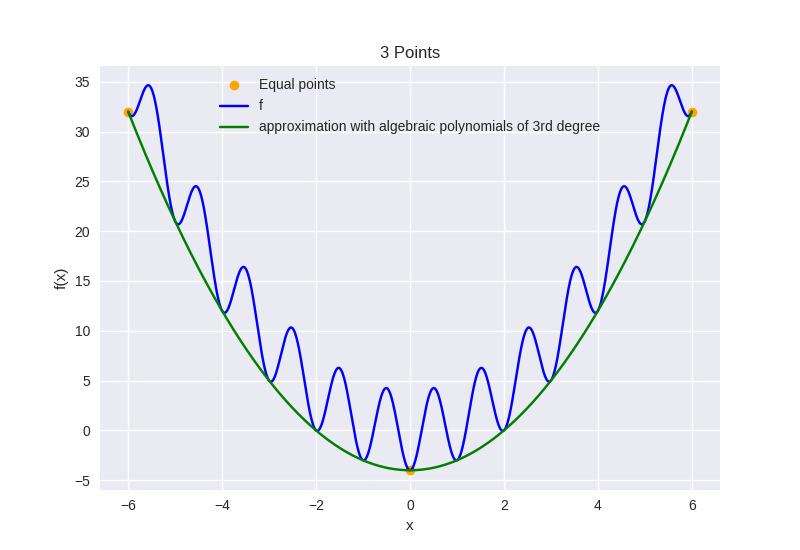
\includegraphics[width=0.9\textwidth]{img/algpoly_2_3.png}
    \caption{Aproksymacja średniokwadratowa wielomianami algebraicznymi 2 stopnia}
\end{figure}

\begin{figure}[H]
    \centering
    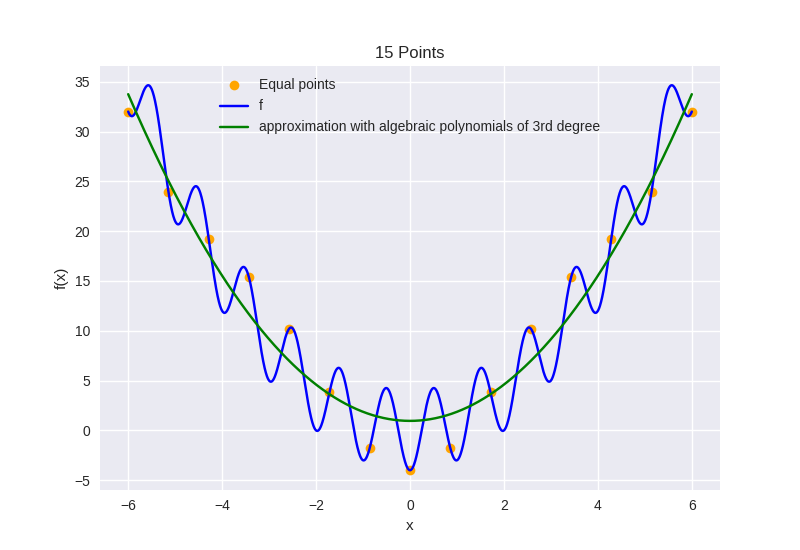
\includegraphics[width=0.9\textwidth]{img/algpoly_2_15.png}
    \caption{Aproksymacja średniokwadratowa wielomianami algebraicznymi 2 stopnia}
\end{figure}

Dla niewielkich stopni wielomianu funkcja aproksymująca nie jest w stanie odtworzyć charakterystycznych "zębów" funkcji aproksymowanej,
jest bardzo wygładzona, niezależnie od liczby punktów. Jedynie zaobserwować można przesuwanie się "paraboli" względem osi $y$.

\begin{figure}[H]
    \centering
    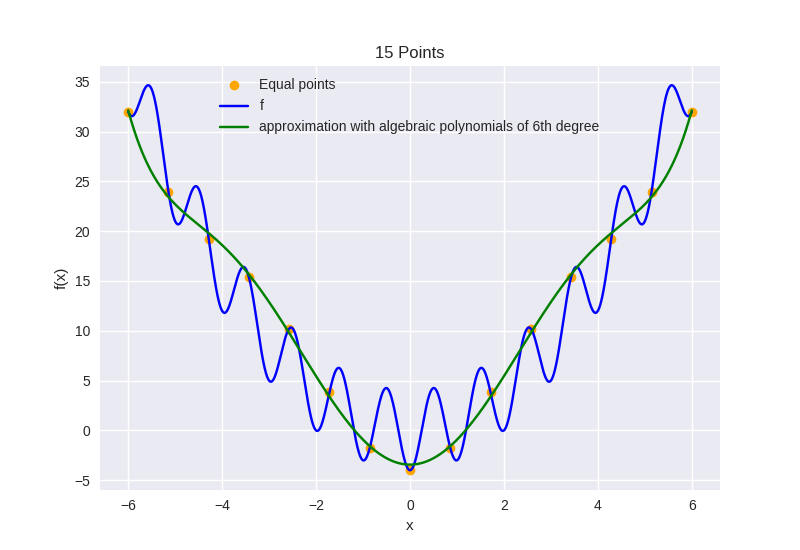
\includegraphics[width=\textwidth]{img/algpoly_6_15.png}
    \caption{Aproksymacja średniokwadratowa wielomianami algebraicznymi 6 stopnia}
\end{figure}

Przy zwiększeniu stopnia wielomianu do szóstego, wykres funkcji zaczyna odbiegać od kształtu paraboli dla niewielkich liczb punktów (np.
na powyższym wykresie), jednak ostatecznie, dla dużych wartości, nadal jest mocno wygładzony i nie odwzorowuje zbyt dokładnie funkcji
$f$, co nie jest zaskakujące, ponieważ stopień wielomianów nadal jest niski.

\begin{figure}[H]
    \centering
    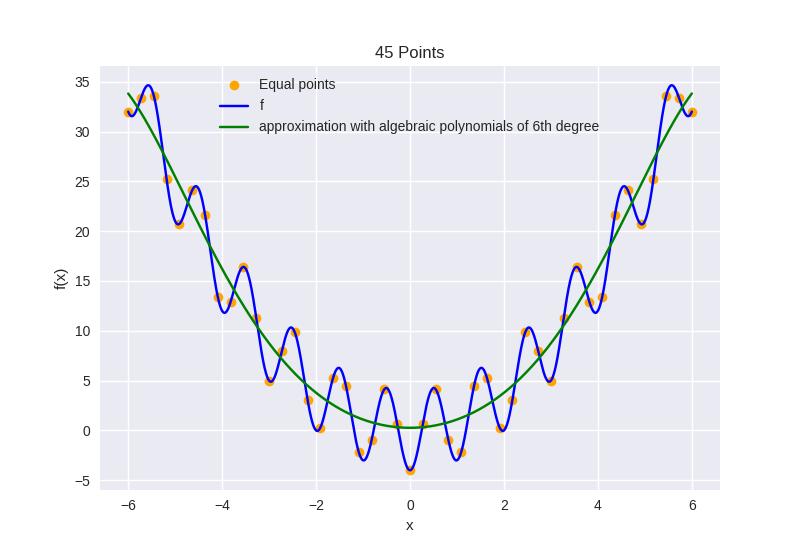
\includegraphics[width=\textwidth]{img/algpoly_6_45.png}
    \caption{Aproksymacja średniokwadratowa wielomianami algebraicznymi 6 stopnia}
\end{figure}

Podobnie dla wielomianów dwunastego stopnia, dla niskich liczb węzłów (12-20) odrobinę bardziej przypominają funkcję $f$ niż wielomiany 
niższego stopnia, a wraz ze  zwiększaniem liczby węzłów, wygładzają się, ponieważ stopień wielomianu jest zbyt niski, 
żeby odwzorować funkcję $f$ dokładniej.

\begin{figure}[H]
    \centering
    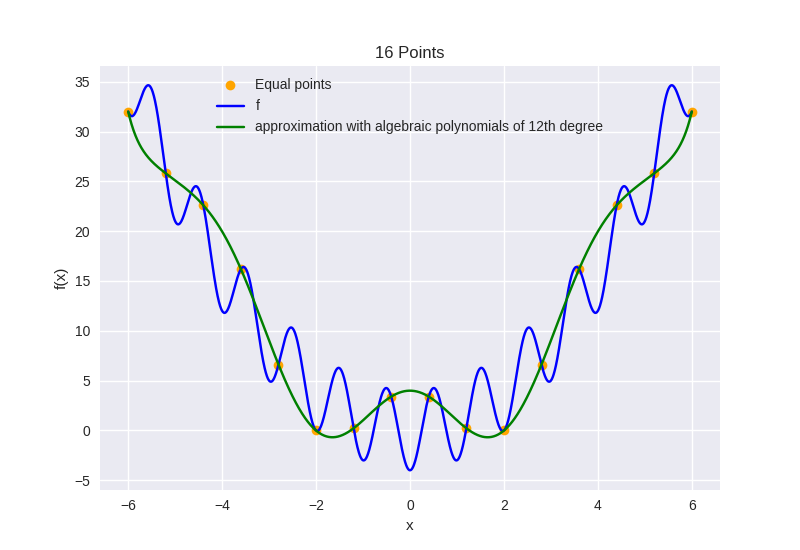
\includegraphics[width=0.8\textwidth]{img/algpoly_12_16.png}
    \caption{Aproksymacja średniokwadratowa wielomianami algebraicznymi 12 stopnia}
\end{figure}

\begin{figure}[H]
    \centering
    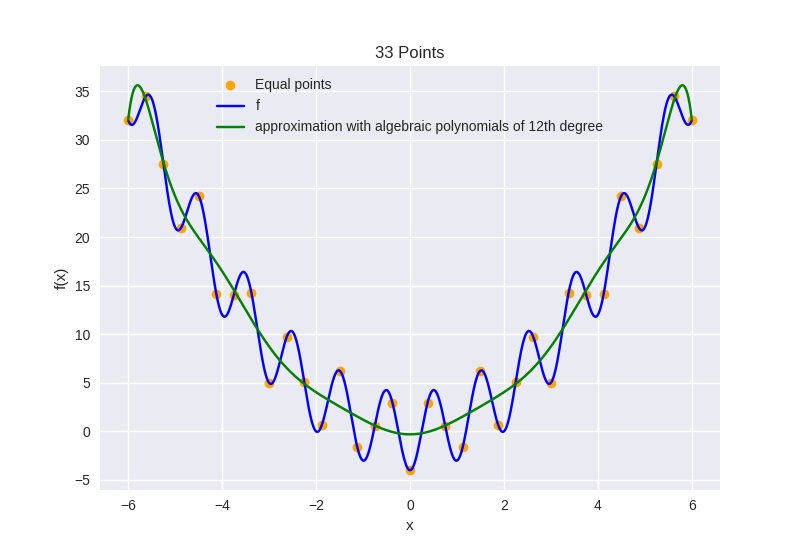
\includegraphics[width=0.8\textwidth]{img/algpoly_12_33.png}
    \caption{Aproksymacja średniokwadratowa wielomianami algebraicznymi 12 stopnia}
\end{figure}

Dla wielomianów wyższych stopni pojawia się efekt Rungego: znaczne pogorszenie dokładności na krańcach przedziału.
Wielomiany dwudziestego stopnia dla niewielkich liczb węzłów obrazują ten efekt, który zmniejsza się jednak wraz ze zwiększaniem
liczby węzłów.

\begin{figure}[H]
    \centering
    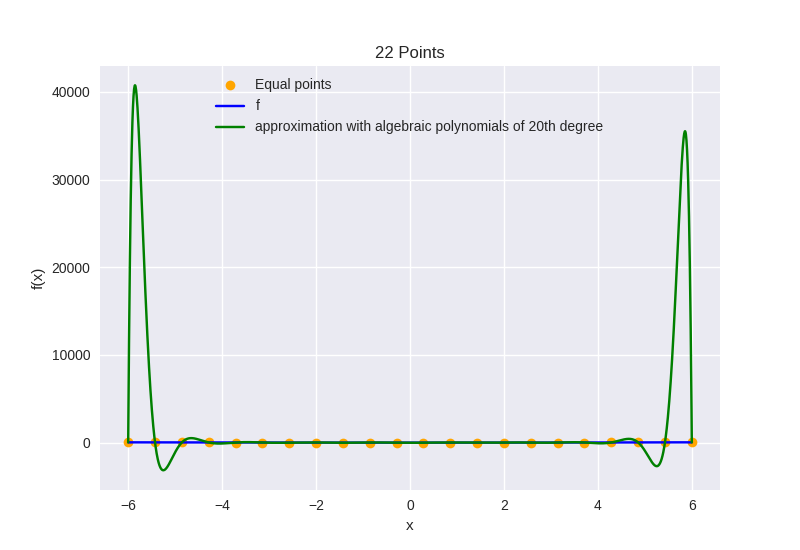
\includegraphics[width=\textwidth]{img/algpoly_20_22.png}
    \caption{Aproksymacja średniokwadratowa wielomianami algebraicznymi 20 stopnia}
\end{figure}

\begin{figure}[H]
    \centering
    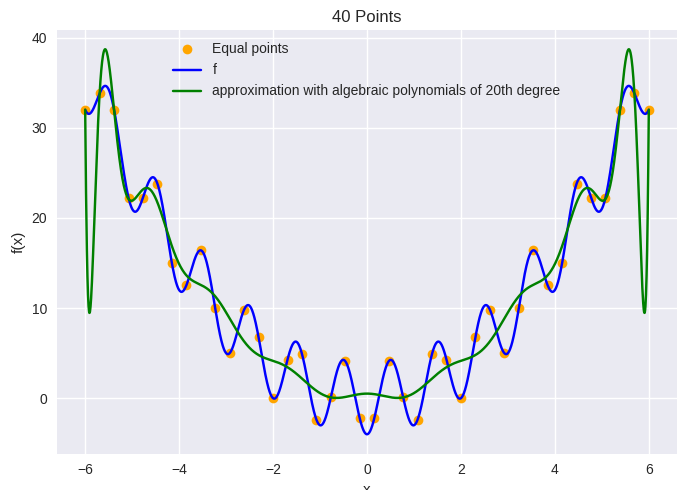
\includegraphics[width=0.8\textwidth]{img/algpoly_20_40.png}
    \caption{Aproksymacja średniokwadratowa wielomianami algebraicznymi 20 stopnia}
\end{figure}


\begin{figure}[H]
    \centering
    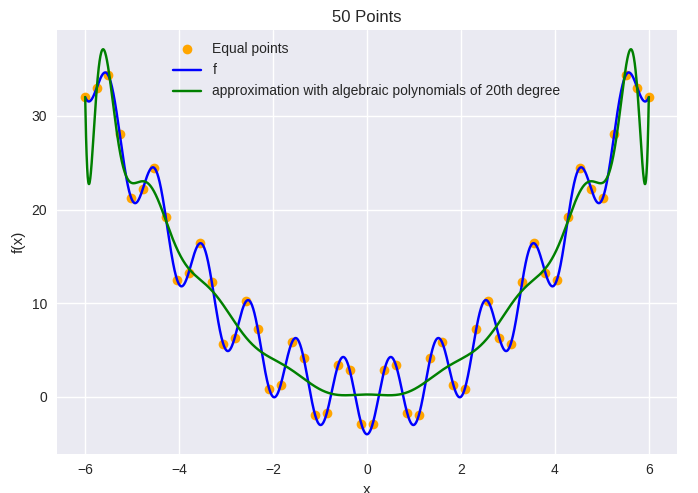
\includegraphics[width=0.8\textwidth]{img/algpoly_20_50.png}
    \caption{Aproksymacja średniokwadratowa wielomianami algebraicznymi 20 stopnia}
\end{figure}

Dla 50 węzłów efekt Rungego jest znacząco mniejszy, niż dla 20.

Przy zastosowaniu wielomianów dużych stopni przetestowane zostało rozłożenie punktów według węzłów Czebyszewa,
które niweluje efekt Rungego.

\begin{figure}[H]
    \centering
    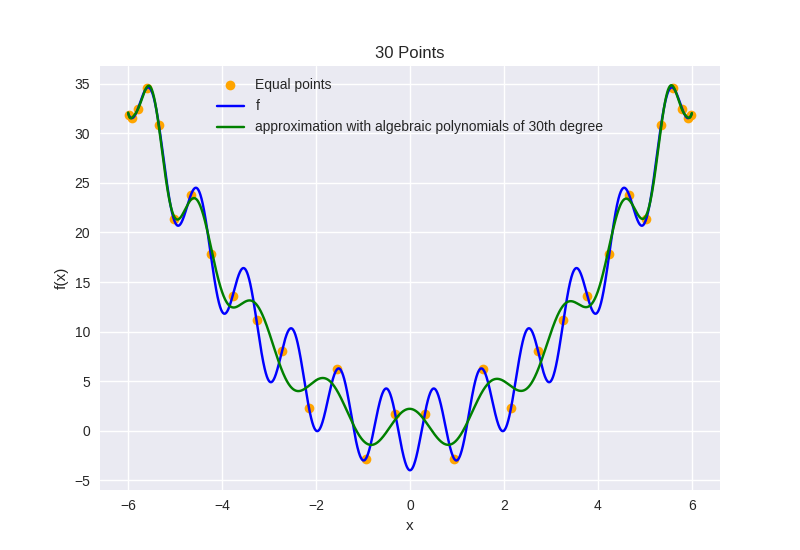
\includegraphics[width=0.8\textwidth]{img/algpoly_30_30.png}
    \caption{Aproksymacja średniokwadratowa wielomianami algebraicznymi 30 stopnia (węzły Czebyszewa)}
\end{figure}

\begin{figure}[H]
    \centering
    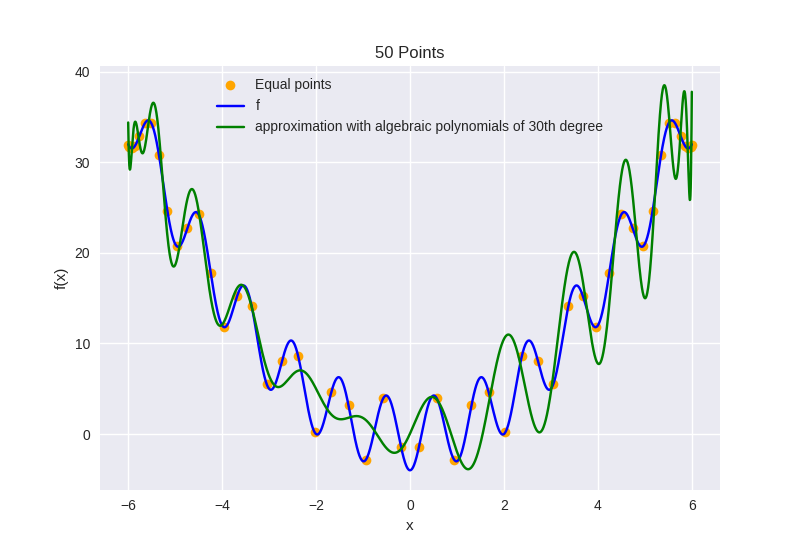
\includegraphics[width=0.8\textwidth]{img/algpoly_30_50.png}
    \caption{Aproksymacja średniokwadratowa wielomianami algebraicznymi 30 stopnia (węzły Czebyszewa)}
\end{figure}

\subsection{Dokładności}
Pozostaje obliczenie dokładności oraz skonfrontowanie wyników z wnioskami uzyskanymi na podstawie analizy wykresów. Miarami dokładności będą:
\begin{itemize}
    \item
    średnia kwadratów odległości wartości wielomianu oraz funkcji $f$ dla 1000 równo oddalonych punktów,
    \item
    maksymalna odległość wartości wielomianu oraz funkcji $f$ dla 1000 równo oddalonych punktów.
\end{itemize}

Pierwszym krokiem będzie zbadanie dokładności dla wielomianów szóstego stopnia przy równomiernie oddalonych punktach.


\begin{table}[H]
\centering
\begin{tabular}{|l|ll|}
\hline
\multicolumn{1}{|c|}{\multirow{2}{*}{\begin{tabular}[c]{@{}c@{}}Liczba\\ węzłów\end{tabular}}} &
    \multicolumn{2}{c|}{Dokładność} \\ \cline{2-3} 
\multicolumn{1}{|c|}{} &
    \multicolumn{1}{c|}{\begin{tabular}[c]{@{}c@{}}Kwad.\\ odl.\end{tabular}} &
    \multicolumn{1}{c|}{\begin{tabular}[c]{@{}c@{}}Maks.\\ odległości.\end{tabular}} \\ \hline
    6 & \multicolumn{1}{l|}{12.502} & 7.072 \\ \hline
    7 & \multicolumn{1}{l|}{23.976} & 8.000 \\ \hline
    8 & \multicolumn{1}{l|}{19.186} & 9.525 \\ \hline
    9 & \multicolumn{1}{l|}{12.197} & 8.686 \\ \hline
    10 & \multicolumn{1}{l|}{9.518} & 6.983 \\ \hline
    11 & \multicolumn{1}{l|}{17.043} & 8.617 \\ \hline
    12 & \multicolumn{1}{l|}{15.975} & 7.993 \\ \hline
    13 & \multicolumn{1}{l|}{23.976} & 8.000 \\ \hline
    14 & \multicolumn{1}{l|}{15.977} & 7.993 \\ \hline
    15 & \multicolumn{1}{l|}{16.462} & 8.356 \\ \hline
    16 & \multicolumn{1}{l|}{8.737} & 5.722 \\ \hline
    17 & \multicolumn{1}{l|}{8.598} & 5.766 \\ \hline
    ... & \multicolumn{1}{l|}{...} & ... \\ \hline
    31 & \multicolumn{1}{l|}{8.024} & 4.550 \\ \hline
    32 & \multicolumn{1}{l|}{8.020} & 4.538 \\ \hline
    33 & \multicolumn{1}{l|}{8.017} & 4.528 \\ \hline
    ... & \multicolumn{1}{l|}{...} & ... \\ \hline
    48 & \multicolumn{1}{l|}{7.990} & 4.449 \\ \hline
    49 & \multicolumn{1}{l|}{7.989} & 4.446 \\ \hline
    50 & \multicolumn{1}{l|}{7.988} & 4.443 \\ \hline
\end{tabular}
\caption{Dokładności dla wielomianów 6 stopnia}
\end{table}

Można zauważyć, że dokładność wzrasta do ok. 16-17 węzłów, potem prawie nie zmienia się aż do liczby 50 węzłów.
Podobne zjawisko zachodzi dla innych niewielkich stopni wielomianu.

\begin{table}[H]
\centering
\begin{tabular}{|l|ll|ll|}
\hline
\multicolumn{1}{|c|}{\multirow{2}{*}{\begin{tabular}[c]{@{}c@{}}Liczba\\ węzłów\end{tabular}}} & \multicolumn{2}{c|}{Równomiernie} & \multicolumn{2}{l|}{Czebyszew} \\ \cline{2-5} 
\multicolumn{1}{|c|}{} &
    \multicolumn{1}{c|}{\begin{tabular}[c]{@{}c@{}}Kwad.\\ odl.\end{tabular}} &
    \multicolumn{1}{c|}{\begin{tabular}[c]{@{}c@{}}Maks.\\ odległości.\end{tabular}} &
    \multicolumn{1}{l|}{\begin{tabular}[c]{@{}l@{}}Kwad.\\ odl.\end{tabular}} &
    \begin{tabular}[c]{@{}l@{}}Maks.\\ odległości.\end{tabular} \\ \hline
    20 & \multicolumn{1}{l|}{611596.723} & 3815.813  & \multicolumn{1}{l|}{13.858}    &   8.803  \\ \hline
    21 & \multicolumn{1}{l|}{1510647.449} & 6367.051 & \multicolumn{1}{l|}{13.127}    &   8.650  \\ \hline
    22 & \multicolumn{1}{l|}{55810386.682} & 40726.485  & \multicolumn{1}{l|}{12.885}    &   8.591  \\ \hline
    23 & \multicolumn{1}{l|}{47.900} & 30.183  & \multicolumn{1}{l|}{12.882}    &   7.916  \\ \hline
    24 & \multicolumn{1}{l|}{139832.401} & 1974.067  & \multicolumn{1}{l|}{12.666}    &   8.452  \\ \hline
    25 & \multicolumn{1}{l|}{43198.463} & 1114.206  & \multicolumn{1}{l|}{11.259}    &   7.269  \\ \hline
    26 & \multicolumn{1}{l|}{11522.581} &  584.943 & \multicolumn{1}{l|}{11.080}    &   8.817  \\ \hline
    27 & \multicolumn{1}{l|}{2464.544} & 272.222  & \multicolumn{1}{l|}{11.279}    &   8.550  \\ \hline
    28 & \multicolumn{1}{l|}{253.958} &  86.182 & \multicolumn{1}{l|}{8.587}    &   6.906  \\ \hline
    29 & \multicolumn{1}{l|}{7.132} & 4.376  & \multicolumn{1}{l|}{7.793}    &   5.938  \\ \hline
    30 & \multicolumn{1}{l|}{40.069} &  35.250 & \multicolumn{1}{l|}{6.709}    &   4.415  \\ \hline
    31 & \multicolumn{1}{l|}{81.173} & 52.016  & \multicolumn{1}{l|}{6.796}    &   4.728  \\ \hline
    32 & \multicolumn{1}{l|}{86.048} &  54.104 & \multicolumn{1}{l|}{6.691}    &   4.488  \\ \hline
    33 & \multicolumn{1}{l|}{76.640} & 51.271  & \multicolumn{1}{l|}{6.716}    &   4.563  \\ \hline
    34 & \multicolumn{1}{l|}{58.043} & 44.426  & \multicolumn{1}{l|}{6.708}    &   4.543  \\ \hline
    35 & \multicolumn{1}{l|}{48.258} & 40.406  & \multicolumn{1}{l|}{6.710}    &   4.547  \\ \hline
    36 & \multicolumn{1}{l|}{39.049} &  36.109 & \multicolumn{1}{l|}{6.710}    &   4.549  \\ \hline
    37 & \multicolumn{1}{l|}{30.772} & 31.568  & \multicolumn{1}{l|}{6.710}    &   4.547  \\ \hline
    38 & \multicolumn{1}{l|}{25.393} & 28.174  & \multicolumn{1}{l|}{6.710}    &   4.547  \\ \hline
    39 & \multicolumn{1}{l|}{20.916} & 24.897  & \multicolumn{1}{l|}{6.710}    &   4.547  \\ \hline
    40 & \multicolumn{1}{l|}{17.581} & 22.084  & \multicolumn{1}{l|}{6.710}    &   4.547  \\ \hline
    41 & \multicolumn{1}{l|}{15.367} & 19.965  & \multicolumn{1}{l|}{6.710}    &   4.546  \\ \hline
    42 & \multicolumn{1}{l|}{13.321} & 17.730  & \multicolumn{1}{l|}{6.710}    &   4.547  \\ \hline
    43 & \multicolumn{1}{l|}{11.989} & 16.107  & \multicolumn{1}{l|}{6.709}    &   4.545  \\ \hline
    44 & \multicolumn{1}{l|}{10.808} & 14.480  & \multicolumn{1}{l|}{6.709}    &   4.544  \\ \hline
    45 & \multicolumn{1}{l|}{9.949} & 13.128  & \multicolumn{1}{l|}{6.710}    &   4.546  \\ \hline
\end{tabular}
\caption{Dokładności dla wielomianów 20 stopnia}
\end{table}

Z tabel wynika, że wzrost stopnia wielomianu bardzo nieznacznie wpływa na dokładność funkcji aproksymującej, natomiast skutkuje
dodatkowymi błędami związanymi z efektem Rungego, które można jednak zniwelować używając innego rozmieszczenia punktów.

\newpage
\section{Wnioski}
Aproksymacja średniokwadratowa wielomianami algebraicznymi jest skutecznym sposobem na przybliżanie funkcji, jeżeli nie musi
być spełniony warunek, że funkcja przybliżające przechodzi przez dane punkty lub jeżeli punkty podane są z błędami (wówczas
interpolacja nie ma sensu). Do aproksymacji można używać wielomianów różnego stopnia, gdzie większe stopnie skutkują nieznaczną
poprawą dokładności, natomiast mniejsze tworzą bardziej gładką funkcję wynikową. Używanie wielomianów wysokich stopni również
może skutować powstawaniem efektu Rungego.

\end{document}